\section{\textbf{Giroscopio}} 
Un giroscopio es un dispositivo utilizado para medir o mantener la orientación y la velocidad angular de un objeto. Su principio de funcionamiento se basa en la conservación del momento angular, lo que le permite detectar cambios en la orientación sin depender de referencias externas. Se emplea en diversas aplicaciones, incluyendo sistemas de navegación inercial, estabilización de vehículos y tecnología aeroespacial.
\subsection{\textbf{Tipos de Giroscopios}}
Existen varios tipos de giroscopios, cada uno con un principio de funcionamiento distinto:

\subsubsection{\textbf{Giroscopios Mecánicos}}
Son compuestos por un rotor que gira rápidamente dentro de un marco o montura.Al girar, el rotor mantiene su orientación debido a la inercia, lo que permite detectar cambios en la posición angular. Se utilizan en aplicaciones como submarinos, aviones y sistemas de estabilización.


\subsubsection{\textbf{Giroscopios Ópticos}}

No tienen partes móviles y funcionan con principios ópticos basados en interferencia de luz. Incluyen los giroscopios de fibra óptica (FOG) y los giroscopios láser de anillo (RLG). Son altamente precisos y se usan en sistemas de navegación de alta precisión, como aeronaves y satélites.


\subsubsection{\textbf{Giroscopios MEMS (Sistemas Microelectromecánicos)}}

Son dispositivos miniaturizados que utilizan la vibración de estructuras internas para detectar cambios en la orientación. Estos s encuentran en teléfonos móviles, drones y dispositivos electrónicos portátiles debido a su pequeño tamaño, bajo costo y eficiencia.


\subsection{\textbf{Funcionamiento del Giroscopio}}
El principio fundamental del giroscopio es la conservación del momento angular, lo que significa que un objeto en rotación mantiene su orientación a menos que una fuerza externa actúe sobre él. Cuando se intenta cambiar la dirección del eje de rotación, el giroscopio responde con un fenómeno llamado precesión, moviéndose en un eje perpendicular a la fuerza aplicada.

En términos matemáticos, la velocidad de precesión se expresa como:

\begin{equation}
	\omega_p = \frac{\tau}{L}
\end{equation}

donde:
\begin{itemize}
	\item $\omega_p$ es la velocidad de precesión,
	\item $\tau$ es el torque aplicado,
	\item $L$ es el momento angular del sistema.
\end{itemize}

En términos prácticos, los giroscopios pueden medir la velocidad angular al detectar la desviación de su rotor o elementos internos con respecto a su posición inicial. En los sistemas ópticos y MEMS, esta medición se realiza mediante sensores electrónicos que convierten las variaciones en señales eléctricas para su procesamiento.

\subsection{\textbf{Aplicaciones del Giroscopio}}
Los giroscopios tienen una amplia gama de aplicaciones en diferentes industrias:

\begin{itemize}
	\item \textbf{Navegación inercial:} En aviones, barcos y submarinos, los giroscopios permiten mantener la orientación sin depender de señales externas como el GPS.
	\item \textbf{Tecnología aeroespacial:} Se emplean en satélites y naves espaciales para el control de actitud y estabilización.
	\item \textbf{Electrónica de consumo:} Se encuentran en teléfonos inteligentes, consolas de videojuegos y cámaras para detectar movimientos y mejorar la experiencia del usuario.
	\item \textbf{Vehículos autónomos y drones:} Ayudan a mantener la estabilidad y orientación durante el movimiento.
\end{itemize}
\begin{figure}[H]
	\centering
	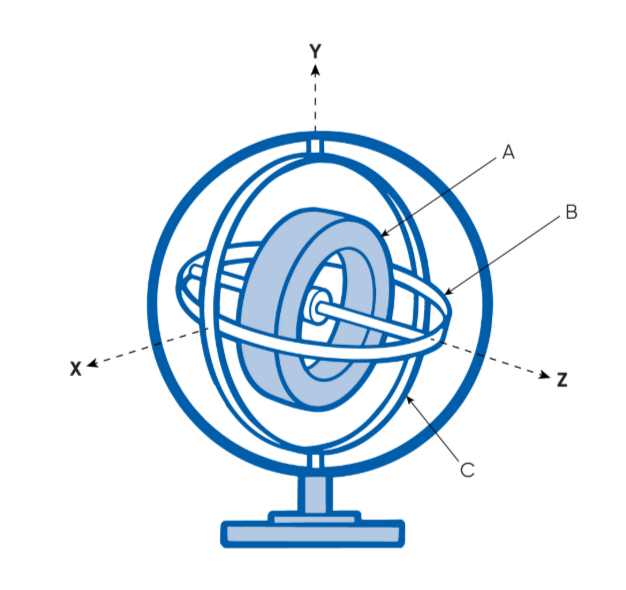
\includegraphics[width=0.35\textwidth]{giroscopio.png}
	\caption{Giroscopio}
\end{figure}